\subsection{Scaled boundary finite element method in 2D elasticity}
\paragraph{}
The SBFEM is reviewed briefly in this section for two-dimensional elasticity.
Detailed derivation can be found in literature \cite{Wolf1996, WOLF20015551, Deeks2002}.
In the SBFEM, a scaling center O is selected at a point from which the whole boundary of the domain is visible (scaling requirement) (see Fig.~\ref{lr_fig:nurbs_rational_basis}).
The boundary of the domain can be represented with conventional finite elements as shown in Fig.~\ref{lr_fig:nurbs_rational_basis}.
The geometry of the domain has only to satisfy the scaling requirement.
This condition is automatically satisfied for all convex polygons and many concave polygons.
The scaling requirement is equivalent to the notion of `star convexity' \cite{Bishop2014}.
For the domain that does not meet the scaling requirement, the requirement can always be satisfied by sub-structuring, i.e. dividing the structure into smaller subdomains, for example, scaled boundary polygon formulation \cite{NATARAJAN2014101}.
\begin{figure}[!ht]
    \centering
    \scalebox{0.4}{
        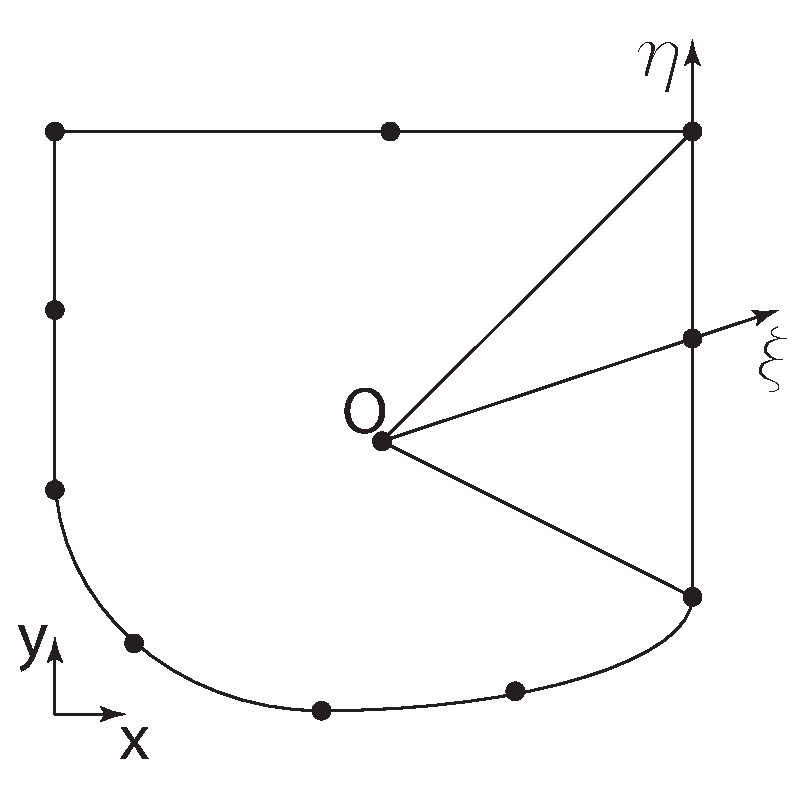
\includegraphics{literature/images/lr_sbfem_desc.eps}
    }
    \label{lr_fig:sbfem_desc}
    \caption{Two dimensional scaled boundary coordinates, where O is the scaling center and $\xi$ is the radial coordinate with $\xi=0$ at the scaling center and $\xi=1$ on the boundary.}
\end{figure}

